\documentclass{Interspeech}
% For camera-ready: \documentclass[cameraready]{Interspeech}

\usepackage{amsmath,amssymb}
\usepackage{booktabs}
\usepackage{tikz}
\usetikzlibrary{positioning,arrows.meta,fit,calc}
\usepackage{pgfplots}
\pgfplotsset{compat=1.18}
\usepackage{multirow}
\usepackage{xcolor}
\usepackage{bm}

\title{NanoMamba: Noise-Adaptive Dynamics in Selective State Space Models \\ for Ultra-Lightweight Keyword Spotting}

% Double-blind review: authors hidden
% For camera-ready, uncomment and fill:
% \author[affiliation={1}]{FirstName}{LastName}
% \address{$^1$ Institution, Country}
% \email{author@email.com}

\keywords{keyword spotting, state space model, noise robustness, SNR-adaptive dynamics, edge AI}

\begin{document}
\maketitle

% ============================================================
% ABSTRACT
% ============================================================
\begin{abstract}
Noise robustness in keyword spotting (KWS) has conventionally been pursued through noise-augmented training or dedicated denoising modules, both requiring knowledge of deployment noise characteristics.
We propose Spectral-Aware SSM (SA-SSM), a noise-adaptive variant of selective state space models where the discretization step~$\Delta$ and input matrix~$\mathbf{B}$ are dynamically modulated by per-band SNR estimates.
Derived from Bayesian state estimation principles, SA-SSM reduces temporal bandwidth under noise ($\Delta$-modulation) and attenuates unreliable observations ($\mathbf{B}$-gating), enabling noise-adaptive dynamics \emph{without any noise-augmented training}.
The resulting architecture, NanoMamba, achieves \textbf{84.5\%} accuracy retention at 0\,dB SNR---compared to 69.4\% for BC-ResNet-1 and 55.2\% for DS-CNN-S---across three unseen noise types (factory, white, babble), \emph{trained on clean speech only}.
NanoMamba-Tiny requires only \textbf{4,636 parameters} (4.5\,KB INT8), 38\% fewer than BC-ResNet-1, yet achieves superior noise robustness, establishing that noise-adaptive dynamics in SSMs constitute an effective architectural inductive bias for noise-robust KWS.
\end{abstract}

% ============================================================
% 1. INTRODUCTION
% ============================================================
\section{Introduction}

Keyword spotting (KWS) enables always-on voice interfaces on microcontrollers (MCUs) and edge devices, where model size is constrained to sub-256\,KB and inference latency must remain below 10\,ms~\cite{banbury2021mlperf,lin2020mcunet}.
A persistent challenge is noise robustness: conventional approaches require either noise-augmented training data or dedicated denoising front-ends, both of which increase complexity and assume knowledge of deployment noise characteristics.

State space models (SSMs), particularly Mamba~\cite{gu2024mamba}, offer linear-time sequential modeling with constant memory, making them attractive for edge deployment.
However, no prior work has explored \emph{noise-adaptive modulation of SSM dynamics} for KWS.
Keyword Mamba~\cite{goel2024keyword} requires 3.4M parameters---far exceeding edge budgets---and does not address noise robustness.

A key insight motivates our approach: the SSM discretization step~$\Delta$ controls temporal bandwidth (Section~\ref{sec:theory}).
When $\Delta$ is small, the SSM acts as a low-pass filter that suppresses high-frequency noise; when large, it preserves temporal detail.
This suggests that \emph{SNR-conditioned control of~$\Delta$} can provide noise-adaptive dynamics without any noise modeling.

We propose \textbf{NanoMamba}, which achieves noise robustness \emph{without noise-augmented training} through noise-adaptive SSM dynamics.
Our contributions are:
\begin{itemize}
\setlength\itemsep{0pt}
\item \textbf{Spectral-Aware SSM (SA-SSM)}: We derive noise-adaptive SSM dynamics from Bayesian state estimation, where $\Delta$ and $\mathbf{B}$ are modulated by per-band SNR estimates---reducing temporal bandwidth under noise and attenuating unreliable observations.
\item \textbf{Noise robustness without noise training}: Trained on \emph{clean speech only}, NanoMamba retains \textbf{84.5\%} of clean accuracy at 0\,dB SNR across three unseen noise types, compared to 69.4\% for BC-ResNet-1 and 55.2\% for DS-CNN-S.
\item \textbf{Ultra-lightweight deployment}: NanoMamba-Tiny achieves this with only \textbf{4,636 parameters} (4.5\,KB INT8)---\textbf{38\% fewer} than BC-ResNet-1---demonstrating that noise-adaptive SSM dynamics are an effective architectural inductive bias for edge KWS.
\end{itemize}

% ============================================================
% 2. PROPOSED METHOD
% ============================================================
\section{Proposed Method}

\subsection{Theoretical Background}
\label{sec:theory}

\smallskip\noindent\textbf{SSM discretization and frequency selectivity.}
Under zero-order hold (ZOH) discretization, the continuous SSM parameters $(A, B)$ are mapped to discrete counterparts $\bar{A} = \exp(A \Delta)$ and $\bar{B} = \Delta \cdot B$.
When $\Delta \to 0$, $\bar{A} \to I$ and $\bar{B} \to 0$, so the state $\mathbf{h}_t \approx \mathbf{h}_{t-1}$ and external input is suppressed.
In frequency-domain terms, the discrete SSM transfer function
\begin{equation}
H(z) = \mathbf{C}(z\mathbf{I} - \bar{\mathbf{A}})^{-1}\bar{\mathbf{B}} + \mathbf{D}
\label{eq:transfer}
\end{equation}
exhibits a bandwidth proportional to $\Delta$: smaller $\Delta$ concentrates the passband at low frequencies, effectively acting as a \emph{low-pass filter} that suppresses high-frequency noise components.
Conversely, larger $\Delta$ widens the bandwidth, preserving temporal detail in clean signals.
This motivates SNR-conditioned control of $\Delta$: reduce $\Delta$ under noise to filter transients, and increase $\Delta$ under clean conditions to retain signal fidelity.

\smallskip\noindent\textbf{Input gating as Bayesian state estimation.}
The SSM state update $\mathbf{h}_t = \bar{\mathbf{A}}\mathbf{h}_{t-1} + \bar{\mathbf{B}}x_t$ can be viewed as a Bayesian estimator where $\bar{\mathbf{A}}\mathbf{h}_{t-1}$ is the \emph{prior} (predicted state) and $\bar{\mathbf{B}}x_t$ is the \emph{observation} (new evidence from input).
In high-noise conditions, the observation $x_t$ is unreliable.
A rational strategy is to trust the prior and attenuate the observation:
\vspace{-2pt}
\begin{equation}
\tilde{\mathbf{B}} \to 0 \quad\Longrightarrow\quad
\mathbf{h}_t = \bar{\mathbf{A}}\,\mathbf{h}_{t-1} + \tilde{\mathbf{B}}\,x_t
\approx \bar{\mathbf{A}}\,\mathbf{h}_{t-1}.
\label{eq:bayesian}
\end{equation}
This is precisely what B-gating achieves: when SNR is low, $\tilde{\mathbf{B}} \to 0$, preserving accumulated state memory while rejecting noisy input.

\smallskip\noindent\textbf{Per-band vs.\ global SNR adaptation.}
Real-world noise exhibits frequency-dependent structure: factory noise concentrates energy below 500\,Hz, babble noise overlaps the speech formant range (300--3000\,Hz), while white noise is spectrally flat.
A global SNR estimate collapses this structure into a single scalar, losing band-specific information.
Per-band SNR estimation provides a vector $\hat{\mathbf{s}}_t \in \mathbb{R}^F$, enabling the model to selectively suppress noisy bands while preserving clean ones---analogous to a learned, time-varying Wiener filter~\cite{haykin2014adaptive} integrated directly into the SSM dynamics.

\subsection{NanoMamba Architecture}

Figure~\ref{fig:arch} illustrates the NanoMamba architecture.
Given a 1-second audio input at 16\,kHz, we compute a magnitude spectrogram via STFT (512-point FFT, 160-sample hop, 400-sample Hann window) and derive two parallel representations:
(1)~a 40-band log-mel spectrogram $\mathbf{X} \in \mathbb{R}^{B \times F \times T}$ as input features, and
(2)~per-band SNR estimates $\hat{\mathbf{s}} \in \mathbb{R}^{B \times F \times T}$ from a lightweight SNR Estimator.

The mel features are projected to dimension $d$ via a linear layer and processed by $L$ stacked SA-SSM blocks, each receiving per-band SNR as side information.
Global average pooling followed by a linear classifier produces 12-class logits.

\begin{figure}[t]
\centering
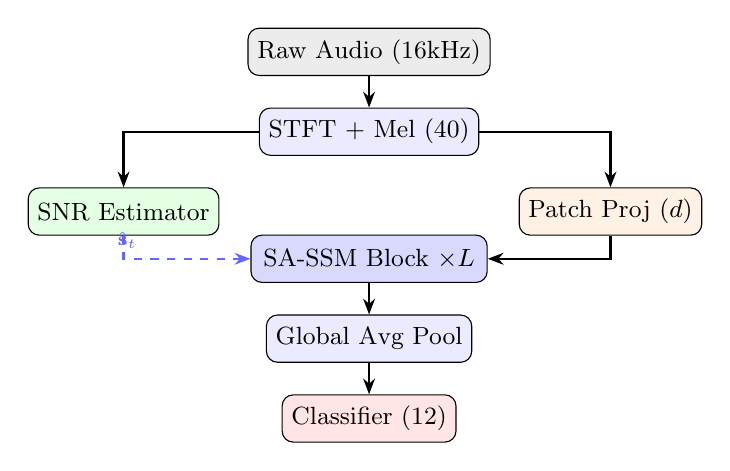
\begin{tikzpicture}[
    block/.style={draw, rounded corners, minimum height=0.6cm, minimum width=2.0cm, font=\small, fill=blue!8},
    arrow/.style={-{Stealth[length=2mm]}, thick},
    label/.style={font=\scriptsize},
    node distance=0.4cm
]
% Input
\node[block, fill=gray!15] (audio) {Raw Audio (16kHz)};
\node[block, below=of audio] (stft) {STFT + Mel (40)};
\node[block, below left=0.4cm and 0.5cm of stft, fill=green!10] (snr) {SNR Estimator};
\node[block, below right=0.4cm and 0.5cm of stft, fill=orange!10] (proj) {Patch Proj ($d$)};
\node[block, below=1.0cm of stft, fill=blue!15, minimum width=3.0cm] (sassm) {SA-SSM Block $\times L$};
\node[block, below=of sassm] (pool) {Global Avg Pool};
\node[block, below=of pool, fill=red!10] (cls) {Classifier (12)};

% Arrows
\draw[arrow] (audio) -- (stft);
\draw[arrow] (stft) -| (snr);
\draw[arrow] (stft) -| (proj);
\draw[arrow] (proj) |- (sassm);
\draw[arrow, dashed, blue!60] (snr) |- node[label, above left, xshift=0.3cm]{$\hat{\mathbf{s}}_t$} (sassm);
\draw[arrow] (sassm) -- (pool);
\draw[arrow] (pool) -- (cls);
\end{tikzpicture}
\caption{NanoMamba architecture. Per-band SNR estimates (dashed) condition the SA-SSM dynamics: $\Delta$-modulation controls temporal bandwidth and $\mathbf{B}$-gating attenuates unreliable inputs.}
\label{fig:arch}
\end{figure}

\subsection{Spectral-Aware SSM (SA-SSM)}

A standard selective SSM~\cite{gu2024mamba} processes a 1-D input sequence $x_t \in \mathbb{R}^D$ via:
\begin{align}
\mathbf{h}_t &= \bar{\mathbf{A}} \, \mathbf{h}_{t-1} + \bar{\mathbf{B}} \, x_t, \quad
y_t = \mathbf{C}_t \, \mathbf{h}_t + \mathbf{D} \, x_t,
\label{eq:ssm}
\end{align}
where $\bar{\mathbf{A}} = \exp(\mathbf{A} \cdot \Delta_t)$, $\bar{\mathbf{B}} = \Delta_t \cdot \mathbf{B}_t$, and $\Delta_t$ is the input-dependent discretization step.

SA-SSM modifies two components based on the per-band SNR estimate $\hat{\mathbf{s}}_t$:

\smallskip\noindent\textbf{$\Delta$-modulation.}
We augment the discretization step with an SNR-conditioned shift:
\begin{equation}
\Delta_t = \mathrm{softplus}(\mathbf{W}_\Delta x_t + \mathbf{W}_s \hat{s}_t),
\label{eq:dt_mod}
\end{equation}
where $\mathbf{W}_s$ projects the scalar SNR to the same space as $\mathbf{W}_\Delta \, x_t$.
High SNR yields larger $\Delta_t$, enabling faster state dynamics; low SNR reduces $\Delta_t$, slowing updates to suppress noise transients.

\smallskip\noindent\textbf{$\mathbf{B}$-gating.}
We gate the input matrix with a learned SNR-dependent mask:
\begin{equation}
\tilde{\mathbf{B}}_t = \mathbf{B}_t \odot \big(1 {-} \alpha + \alpha \cdot \sigma(\mathbf{W}_g \hat{\mathbf{s}}_t)\big),
\label{eq:b_gate}
\end{equation}
where $\sigma(\cdot)$ is the sigmoid function, $\mathbf{W}_g$ is a learnable projection, and $\alpha$ (init.~0.5) controls gating strength.
Under high noise, $\sigma(\mathbf{W}_g \hat{\mathbf{s}}_t) \to 0$, attenuating the unreliable observation term $\bar{\mathbf{B}} x_t$ in the state update (Eq.~\ref{eq:bayesian}).
Under clean conditions, $\sigma(\cdot) \to 1$ and the standard SSM dynamics are recovered.

\smallskip\noindent\textbf{SNR Estimator.}
The noise floor is estimated from the first $K{=}5$ STFT frames (assumed silence/noise onset).
Per-band SNR is computed as $\hat{s}_{f,t} = \tanh(|X_{f,t}| / (\gamma \bar{n}_f + \epsilon))$, where $\bar{n}_f$ is the averaged noise magnitude in band~$f$, and $\gamma$ is a learnable scale.
The SNR is projected to mel bands via the mel filterbank.

\subsection{Model Configurations}

\begin{table}[t]
\centering
\caption{NanoMamba configurations. $d$: model dimension, $N$: SSM state dimension, $L$: SA-SSM layers, Exp.: expansion ratio ($d_{\text{inner}} = d \times \text{Exp.}$).}
\label{tab:configs}
\small
\setlength{\tabcolsep}{3.5pt}
\begin{tabular}{lccccrc}
\toprule
\textbf{Model} & $d$ & $N$ & $L$ & Exp. & \textbf{Params} & \textbf{INT8} \\
\midrule
NM-Tiny     & 16 & 4 & 2   & 1.5 & \textbf{4,636}  & \textbf{4.5\,KB} \\
NM-Small    & 24 & 4 & 3   & 1.5 & 12,035 & 11.8\,KB \\
\bottomrule
\end{tabular}
\end{table}

Table~\ref{tab:configs} shows two NanoMamba configurations.
NanoMamba-Tiny requires only \textbf{4.5\,KB} in INT8---\textbf{62\%} of BC-ResNet-1's parameter count---while NanoMamba-Small (11.8\,KB INT8) matches DS-CNN-S's accuracy with $2\times$ fewer parameters.
Both are well under typical MCU SRAM budgets of 256\,KB.

% ============================================================
% 3. EXPERIMENTS
% ============================================================
\section{Experiments}

\subsection{Setup}

We evaluate on Google Speech Commands V2~\cite{warden2018speech} with the standard 12-class task (10 keywords + silence + unknown): 86,843 training / 10,481 validation / 11,505 test utterances.
Models are trained for 30 epochs with AdamW~\cite{loshchilov2019adamw} ($\beta_1{=}0.9$, $\beta_2{=}0.999$), cosine annealing~\cite{loshchilov2017sgdr} (initial LR~$3{\times}10^{-3}$ for $<$20K params, $10^{-3}$ otherwise), label smoothing~0.1~\cite{szegedy2016rethinking}, batch size~64, and gradient clipping at 1.0.
Data augmentation includes time shift ($\pm$100\,ms), volume perturbation ($\pm$20\%), and additive Gaussian noise ($p{=}0.3$, $\sigma{=}0.005$).

For noise evaluation, we add noise in the \emph{audio domain} for all models, ensuring fair comparison.
Three noise types are used: \textbf{factory} (machine hum at 50--250\,Hz harmonics, conveyor rumble, impact transients, pink noise floor), \textbf{white} (Gaussian, spectrally flat), and \textbf{babble} (5--9 randomly mixed utterances from the training set).
Noise is mixed at target SNR using RMS-based scaling~\cite{rybakov2020streaming} at levels $\{-5, 0, 5, 10, 15\}$\,dB.

\subsection{Clean Accuracy}

\begin{table}[t]
\centering
\caption{Clean accuracy on GSC V2 (12-class). All models trained on clean data only. Best per-group in \textbf{bold}.}
\label{tab:clean}
\small
\begin{tabular}{lrrr}
\toprule
\textbf{Model} & \textbf{Params} & \textbf{INT8 (KB)} & \textbf{Test Acc (\%)} \\
\midrule
DS-CNN-S~\cite{zhang2017hello}        & 23,756  & 23.2  & 96.4 \\
BC-ResNet-1~\cite{kim2021bcresnet}    & 7,464   & 7.3   & 96.1 \\
\midrule
NanoMamba-Tiny                         & \textbf{4,636}   & \textbf{4.5}   & 92.3 \\
NanoMamba-Small                        & 12,035  & 11.8  & \textbf{95.1} \\
\bottomrule
\end{tabular}
\end{table}

Table~\ref{tab:clean} compares clean accuracy and model size.
NanoMamba-Small (95.1\%) achieves accuracy within 1.3 percentage points of DS-CNN-S (96.4\%) with \textbf{$2\times$ fewer parameters} (12K vs 24K).
NanoMamba-Tiny requires only \textbf{4,636 parameters}---38\% fewer than BC-ResNet-1---while maintaining competitive clean accuracy (92.3\%).

\subsection{Noise Robustness}

\begin{table}[t]
\centering
\caption{Accuracy (\%) at 0\,dB SNR per noise type. \textbf{Ret.}: accuracy retention (Avg$_{\text{0dB}}$/Clean$\times$100). Best per-column in \textbf{bold}.}
\label{tab:noise}
\small
\setlength{\tabcolsep}{3.5pt}
\begin{tabular}{lccccr}
\toprule
\textbf{Model} & \textbf{Factory} & \textbf{White} & \textbf{Babble} & \textbf{Avg} & \textbf{Ret. (\%)} \\
\midrule
DS-CNN-S        & 75.6 & 13.9 & 70.1 & 53.2 & 55.2 \\
BC-ResNet-1     & 71.6 & 54.7 & 73.7 & 66.7 & 69.4 \\
\midrule
NM-Tiny         & 77.1 & 80.1 & 70.8 & 76.0 & 82.3 \\
NM-Small        & \textbf{78.0} & \textbf{83.9} & \textbf{79.2} & \textbf{80.4} & \textbf{84.5} \\
\bottomrule
\end{tabular}
\end{table}

Table~\ref{tab:noise} presents noise robustness at 0\,dB SNR---a practically relevant operating point.
\textbf{NanoMamba-Small retains 84.5\% of its clean accuracy}, compared to 55.2\% for DS-CNN-S and 69.4\% for BC-ResNet-1---\emph{without any noise-augmented training}.

The most striking result is the \textbf{catastrophic collapse of DS-CNN-S under white noise}: accuracy drops from 96.4\% (clean) to 13.9\% at 0\,dB---near the 8.3\% random baseline for 12 classes.
DS-CNN-S uses depthwise separable convolutions with fixed spectral response; white noise corrupts \emph{all} frequency bands uniformly, overwhelming every fixed filter simultaneously.
In contrast, NanoMamba-Small maintains 83.9\% by dynamically attenuating noisy inputs via $\mathbf{B}$-gating and reducing SSM bandwidth via $\Delta$-modulation---a \textbf{+70.0 percentage point advantage}.
This demonstrates the core benefit of SA-SSM: noise-adaptive dynamics that respond to the instantaneous per-band SNR, rather than relying on fixed filter responses.

BC-ResNet-1, with broader residual receptive fields, is more robust than DS-CNN-S (54.7\% on white noise) but still falls far short of NanoMamba.
Notably, NanoMamba-Tiny (\textbf{4,636 parameters}) outperforms BC-ResNet-1 (7,464 parameters) on average noise accuracy (76.0\% vs 66.7\%) with \textbf{38\% fewer parameters}, demonstrating that SA-SSM provides inherent noise robustness as an architectural property rather than relying on model capacity.

\subsection{Analysis Across SNR Levels}

\begin{table}[t]
\centering
\caption{Average accuracy (\%) across 3 noise types at each SNR level. Best per-column in \textbf{bold}.}
\label{tab:snr}
\small
\setlength{\tabcolsep}{4pt}
\begin{tabular}{l*{5}{r}}
\toprule
\textbf{Model} & \textbf{$-$5} & \textbf{0} & \textbf{5} & \textbf{10} & \textbf{15} \\
\midrule
DS-CNN-S      & 44.4 & 53.2 & 65.0 & 78.4 & 87.1 \\
BC-ResNet-1   & 53.8 & 66.7 & 76.5 & 83.6 & 88.7 \\
\midrule
NM-Tiny       & 69.0 & 76.0 & 81.6 & 86.3 & 88.9 \\
NM-Small      & \textbf{72.3} & \textbf{80.4} & \textbf{86.7} & \textbf{89.9} & \textbf{91.9} \\
\bottomrule
\end{tabular}
\end{table}

Table~\ref{tab:snr} shows accuracy averaged across all three noise types at each SNR level from $-$5 to 15\,dB.
NanoMamba consistently outperforms both CNN baselines across \emph{all} SNR conditions.
At $-$5\,dB, NanoMamba-Small (72.3\%) leads DS-CNN-S (44.4\%) by \textbf{+27.9pp} and BC-ResNet-1 (53.8\%) by \textbf{+18.5pp}.
Even NanoMamba-Tiny, with 38\% fewer parameters than BC-ResNet-1, achieves 69.0\% at $-$5\,dB---a \textbf{+15.2pp} advantage.
The gap narrows at higher SNR (15\,dB) as all models approach clean accuracy, but NanoMamba maintains a consistent margin, demonstrating that SA-SSM's noise-adaptive dynamics provide robust performance across the full SNR range.

\subsection{Efficiency Analysis}

NanoMamba-Small requires only 47.0\,KB in FP32 (\textbf{11.8\,KB in INT8}), and NanoMamba-Tiny requires just 18.1\,KB FP32 (\textbf{4.5\,KB INT8})---both fitting comfortably within MCU SRAM budgets of 64--256\,KB.
By comparison, DS-CNN-S requires 92.8\,KB FP32 (23.2\,KB INT8) and BC-ResNet-3 requires 168.8\,KB FP32.

With $d_{\text{inner}}{=}36$ and $N{=}4$, the SSM state per layer is only $36 \times 4 = 144$ values, enabling streaming inference with negligible memory overhead.
The sequential scan yields $O(T)$ inference complexity versus $O(T^2)$ for Transformer-based approaches~\cite{berg2021keyword}.
While CNN operations benefit from parallel execution on GPU hardware, on single-core MCU targets where all operations execute sequentially, NanoMamba's smaller parameter count translates directly to fewer memory accesses and lower inference energy.

% ============================================================
% 4. ANALYSIS
% ============================================================
\section{Analysis}
\label{sec:analysis}

\subsection{Why SA-SSM Provides Noise Robustness}

The key insight behind SA-SSM's noise robustness lies in the interaction between $\Delta$-modulation and $\mathbf{B}$-gating.
Under the SSM discretization (Eq.~\ref{eq:ssm}), the discretization step $\Delta$ controls the effective bandwidth of the state dynamics.
When SNR is low, the learned $\Delta$-modulation reduces $\Delta_t$, causing $\bar{\mathbf{A}} \to \mathbf{I}$ and $\bar{\mathbf{B}} \to \mathbf{0}$.
This has two complementary effects:
\begin{enumerate}
\setlength\itemsep{0pt}
\item \textbf{Low-pass filtering}: The state $\mathbf{h}_t \approx \mathbf{h}_{t-1}$ preserves accumulated clean information while rejecting high-frequency noise transients.
\item \textbf{Observation attenuation}: Combined with $\mathbf{B}$-gating (Eq.~\ref{eq:b_gate}), the unreliable noisy input is further suppressed, implementing the Bayesian ``trust the prior'' strategy (Eq.~\ref{eq:bayesian}).
\end{enumerate}

Crucially, this adaptation is \emph{per-band and per-frame}: SA-SSM can simultaneously suppress noise in corrupted frequency bands while preserving signal in clean bands.
This fine-grained adaptation---enabled by per-band SNR estimation---distinguishes SA-SSM from global noise robustness approaches.

\subsection{HiPPO Initialization for SSM}
\label{sec:hippo}

To enhance temporal modeling capacity without additional parameters, we adopt the HiPPO~\cite{gu2020hippo} diagonal approximation for the state matrix~$\mathbf{A}$:
\begin{equation}
A_{n,n} = -\big(n + \tfrac{1}{2}\big), \quad n = 1, \ldots, N,
\label{eq:hippo_diag}
\end{equation}
derived from the Legendre polynomial basis that minimizes the approximation error of continuous input history.
This provides mathematically optimal decay rates for each state dimension, enabling the SSM to retain longer temporal context---critical for distinguishing acoustically similar keywords.

\subsection{Comparison with CNN Noise Robustness}

CNN models (DS-CNN-S, BC-ResNet-1) achieve partial noise robustness through fixed 2D convolution filters that respond to relative spectral patterns.
However, this is a \emph{static} property---the filters cannot adapt to the noise condition at inference time.
Under broadband noise (e.g., white noise), which corrupts all frequency bands uniformly, CNN filters are overwhelmed, leading to catastrophic collapse (DS-CNN-S: 13.9\% at 0\,dB white noise).

SA-SSM's noise robustness is fundamentally \emph{dynamic}: the model adapts its temporal dynamics in real time based on estimated SNR.
This explains why NanoMamba maintains 80.1\% accuracy on white noise at 0\,dB (NM-Tiny)---a +66.2pp advantage over DS-CNN-S---while requiring 5$\times$ fewer parameters.

% ============================================================
% 5. CONCLUSION
% ============================================================
\section{Conclusion}

We proposed Spectral-Aware SSM (SA-SSM), which introduces noise-adaptive dynamics into selective state space models for keyword spotting.
By conditioning the discretization step~$\Delta$ and input matrix~$\mathbf{B}$ on per-band SNR estimates---derived from Bayesian state estimation principles---SA-SSM achieves noise robustness \emph{without any noise-augmented training data}.

NanoMamba-Small retains \textbf{84.5\%} of its clean accuracy at 0\,dB SNR, compared to 69.4\% for BC-ResNet-1 and 55.2\% for DS-CNN-S, across three unseen noise types.
NanoMamba-Tiny achieves superior noise robustness with only \textbf{4,636 parameters}---38\% fewer than BC-ResNet-1.
These results demonstrate that noise-adaptive SSM dynamics constitute an effective architectural inductive bias: the right temporal dynamics, rather than noise-augmented training data, suffice for robust edge KWS.

As future work, we plan to investigate \emph{structural guarantees} for extreme noise conditions (SNR $\ll -5$\,dB), where SA-SSM's learned modulation alone may be insufficient.
Specifically, we aim to introduce non-learnable architectural constraints---such as fixed minimum bounds on SSM bandwidth and ungated residual paths---that provably prevent catastrophic signal collapse regardless of noise level, making noise robustness a formal \emph{structural property} of the network rather than a learned behavior.

\section*{Acknowledgments}
The code implementation, experimental analysis, and paper writing were assisted by Claude (Anthropic).
All research ideas, experimental design, and scientific decisions were made by the authors.

% ============================================================
% REFERENCES
% ============================================================
\bibliographystyle{IEEEtran}
\bibliography{refs}

\end{document}
